% !TeX root =./main.tex
% !TeX spellcheck = en_US

Due to a global economic expansion, the transport sector has been gaining massive momentum for years \cite{gungor2018detect}.
Since 2010, global freight volumes continuously increase with forecasts predicting growth rates of 3.2\% per year until 2050 \cite{figura2020preferences, InternationalTransportForum}.
Various transportation modes, including rail, maritime, air, and road, are available to cope with this rapid development and to satisfy future transportation needs.
However, primary focus is generally placed on the road transport segment due to its dominating role for domestic transportation, with almost 80\% of the total volume of goods being carried by trucks in the European Union \cite{Eurostat}.
The increase in demand for transportation also holds true for superheavy, bulky and extra-large goods \cite{gavrilova2021analysis}, referred to as oversized and heavyweight cargoes (\ohc) in this article \cite{Luo.2021}.
\ohc is typically associated with the transportation of industry goods (e.g., generators, turbines, construction equipment) that exceed defined limits in terms of weight and/or size, many of which without permission, i.e, illegally \cite{fiorillo2016minimizing}. This is especially the case for cross-border activities where operators are frequently faced with different legal requirements.
\par In comparison with traditional freight transportation, \ohc requires time-consuming and complex efforts with regard to planning, approval, and execution, as no two \ohc transports are completely the same \cite{Wolnowska.2019}.
Some \ohc transports may require complete road closures or detours and escort by police or other law enforcement.
Consequently, planning is usually conducted on an individual level, taking the respective specifications of each \ohc transport into consideration \cite{Bazaras.2013}.
In doing so, several relevant technical, administrative, and organizational criteria are subject of detailed analysis to reduce economic and social risks as well as political dispute, thereby increasing the general safety and societal acceptance of \ohc transports \cite{Palsaitis.2012}.
Granular planning is further dependent on national legislation and involves the evaluation of multiple factors \cite{zhu2014vehicle}. Oversized load is particularly limited by turns, corridor widths, and obstacles along the road, such as traffic lights or power lines \cite{PETRASKA.2018, arentze2012context}. Heavyweight load, i.e., vehicles loaded with more than 11 tons per axle, is for instance limited by ascents and descents. Safety issues on ascents and descents especially come along with changing road conditions due to heavy rain, snow, or ice. Besides that, exuberant wear and deterioration of the involved means of transport induce extra costs and can cause adverse health effects, e.g., due to excessive amounts of brake dust \cite{Gerlofs2019}. This relates especially to mountainous regions such as the area around the European Alps.
Another safety-relevant attribute that needs to be considered in terms of heavyweight load is the maximum bridge carrying capacity, which must not be surpassed by the total weight of an \ohc transport, and thus, is highly influencing route planning activity.
Excessive overload significantly contributes to shorten service lifes of pavements and bridges as well as it reduces bridge safety to levels that may fall below those set in the design standards, potentially resulting in failures or collapse \cite{fiorillo2018fragility, yan2018optimal, ghosn2000development, wu2019assessment, lou2016effect}. Hence, planning is highly influenced by local characteristics and in-person inspection is required once a particular transport route has been submitted to the authority.
Critical incidents, such as the Genova bridge collapse in 2018 \cite{Morgese.2020, MorandiNYTimes},  demonstrate the effects of long-term exceeding of permitted limits on infrastructure, thereby underlining the importance of complying with certain standards and norms in \ohc planning. However, a cornerstone for ensuring compliance is monitoring via fixed or mobile truck weighing stations \cite{fiorillo2016minimizing}.
\par In practice, the route planning process for \ohc transports involves several stakeholders, such as client companies, carriers, governmental institutions, and civil engineers.
This labor intense planning procedure is described in \cite{Osegueda.1999} and \cite{ray2007web}. In the beginning, the client company or carrier drafts a first route design and submits this draft to the responsible authority for approval.
Subsequently, a civil engineer is consulted to determine route feasibility based on statical calculations and on-site inspections of critical route sections. Apart from the route profile with its potential bottlenecks, ascents and descents, tolerances, technical specifications, and other structural parameters of bridge elements are examined in detail. In case a route is generally feasible, permits are often accompanied by speed restrictions on certain road segments. In the event of route infeasibility due to exceeding of permitted limits or for any other reason, the initial draft needs to be revised, adapted, and resubmitted by the applicant and subsequently re-evaluated by the civil engineer.


\begin{figure}[!ht]
  \centering
  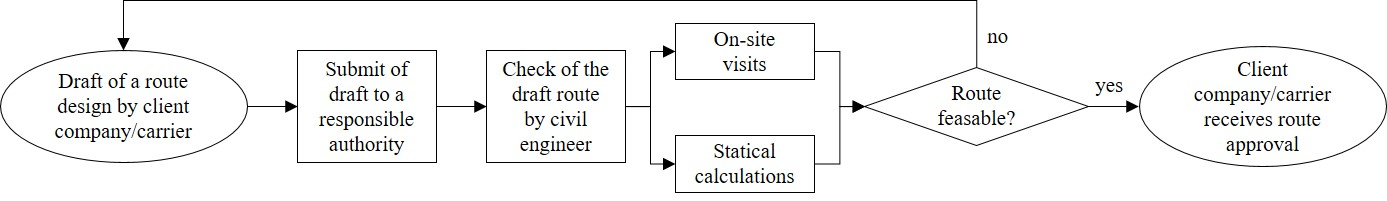
\includegraphics[width=0.9\textwidth]{final.jpg}
  \caption{Main elements of the \ohc transport planning process.}
  \label{fig:higherlevel}
\end{figure}

\begin{figure}[!ht]
  \centering
% !TeX root =../main.tex
% !TeX spellcheck = en_US

% https://www.overleaf.com/learn/latex/LaTeX_Graphics_using_TikZ%3A_A_Tutorial_for_Beginners_(Part_3)%E2%80%94Creating_Flowcharts


\tikzstyle{startstop} = [rectangle, rounded corners, minimum width=1cm, minimum height=1cm,text centered, draw=black, fill=red!30]
\tikzstyle{io} = [trapezium, trapezium left angle=70, trapezium right angle=110, minimum width=1cm, minimum height=1cm, text centered, draw=black, fill=blue!30]
\tikzstyle{process} = [rectangle, minimum width=1cm, minimum height=1cm, text centered, draw=black, fill=orange!30]
\tikzstyle{decision} = [diamond, minimum width=1cm, minimum height=1cm, text centered, draw=black, fill=green!30]
\tikzstyle{arrow} = [thick,->,>=stealth]


\begin{tikzpicture}[node distance=2.5cm, font=\footnotesize]

  \node (start) [startstop] {Draft Route};

    \node (pro1) [process, text width=1.5cm,right of=start] {submit draft to responsible authority};

    \node (pro2) [process, text width=1.5cm, right of=pro1] {check draft by civil engineer};

    \node (pro3) [process, text width=1.5cm, right of=pro2,  yshift=1cm] {On-site visits};
    \node (pro4) [process, text width=1.5cm, right of=pro2,  yshift=-1cm] {Statistical calculations};

    \node (dec1) [decision, text width=1.5cm, right of=pro4, yshift=1cm,  ] {Route Feasible};

    \node (appr) [startstop,  text width=1.5cm, right of=dec1] {Approval Granted};


    \draw [arrow] (start.east) -- (pro1.west);
    \draw [arrow] (pro1.east) -- (pro2.west);
    \draw [arrow] (pro2.east) -- (pro3.west);
    \draw [arrow] (pro2.east) -- (pro4.west);
    \draw [arrow] (pro4.east) -- (dec1.west);
    \draw [arrow] (pro3.east) -- (dec1.west);



    % \draw [arrow] (dec1.east) -- (appr.west);
    \draw [arrow] (dec1.east) -- node[anchor=south] {yes} (appr.west);
    % \draw [arrow] (dec1.north) |- node[anchor=south] {no} (pro1.north);

    \draw [arrow] (dec1.north) -- ([yshift=0.5cm]dec1.north) node [near start] {no}  --    ([yshift=1cm]pro1.north) -| (pro1.north);



    % \draw [arrow] (dec1.north) -- (start.north);

    % \draw [arrow] (dec1) -- node[anchor=south] {no} (pro2b);



  \end{tikzpicture}

  \caption{Main elements of the \ohc transport planning process.}
  \label{fig:higherlevel2}
\end{figure}

This costly and time-consuming process must be repeated until the route is declared feasible and a permit is granted. As of this moment, the approved route must not be deviated from.
What seems to be problematic in this respect is that the development of the initial draft is primarily based on practical experience and commercial GIS applications that are limited in terms of data availability and accuracy.
Standard GIS solutions indeed consider temporary construction sites or road closures but exhibit a severe lack of data on road gradients as well as bridge locations and the respective carrying capacities, and thus, do not facilitate the identification of an optimal route under consideration of weight limits.
Therefore, there is a need of professional software that thoroughly takes weight-related parameters into account.
\par In an attempt to simplify the cumbersome authorization process, we take an optimization approach.
To this end, a mathematical model is used to determine the optimal path between two points within the road network while respecting certain constraints, e.g., in terms of road gradients and weight limits \cite{liedtke2012generation, zhu2014vehicle}.
Under the assumption that the model results in more than one feasible routes, a study that compares several (possibly conflicting) objectives will be conducted.
In doing so, we consider different types of vehicles and loads. The results should provide \textit{decision support} for reducing the complexity of \ohc route planning.
\par
The article continues in section 2 with a review of the existing body of knowledge in the respective field.
In section 3, we provide the problem description and introduce notations along with the model assumptions. In section 4, the optimization model is presented and illustrated in an example of application.
Finally, section 5 closes the article, summarizing the research implications, study limitations, and future lines of research.
